\section{Horn}
The purpose of the horn is to indicate an overtake when coming from behind. The horn is implemented by demand from Shell Eco-Marathon. There are various demands that must followed. The most prolific of these is that the horn must emit a sound higher than 85 dB at 4 meters. For other requirements regarding the horn, see section~\vref{sec:requirements}.  

\subsection{Design}
First off, when designing the horn it was necessary to find a suitable horn, that would be able to match the requirements set forth by Shell. There were various options, but it was chosen to use an electric buzzer. This was done as it was the type of horn using the least amount of current. \\
Next up was the design of output stage. In this design it has been chosen to use a BJT transistor. It is used as a switching transistor, turning on and off according to input signal. There is a base resistance which size is defined by the h\textsubscript{fe} and the current used to supply the horn. \\
\begin{align}
	\begin{split}
		I_b &= \frac{I_c}{h_{fe}}
	\end{split}
\end{align}
Where $I_b$ is the current flowing into the base \\ 
$I_c$ is the current flowing in the collector \\ 
$h_{fe}$ is the beta value of the transistor. \\

Lastly, there is going to some safety implemented. Here in the form of a diode, which supplies a path for return current when the transistor is off. This protection is mostly implemented for use with a magnetic buzzer, but it is implemented so that the PCB is prepared for many different kind of buzzers.   

\subsection{Implementation}
A full overview concerning the controls of the buzzer can be seen on the figure underneath.

\begin{figure}[H]
	\centering
	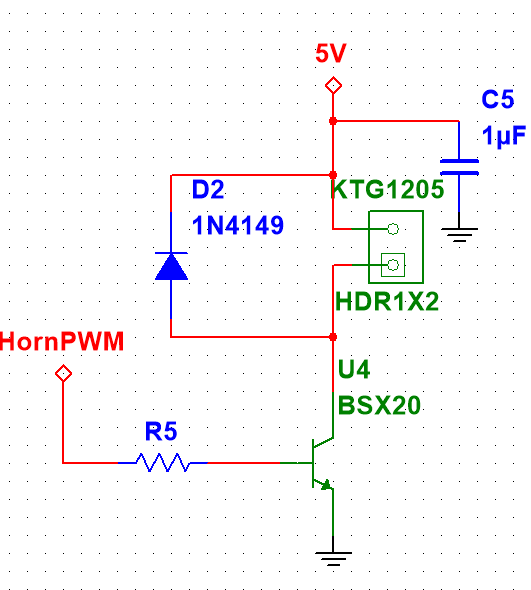
\includegraphics[width=0.7\linewidth]{Hardware/Pictures/Horn_hw}
	\caption{Horn hardware overview}
	\label{fig:Horn_control}
\end{figure}

The specific transistor being used is BSX20.The datasheet \fxnote{Husk ref} for this BJT shows a minimum guaranteed $h_fe$ for these is 40 and therefore that which will be used. This makes the calculations worst case, since the used BJT probably will have a larger $h_fe$. The desired collector current will be set by the buzzer being used and will therefore vary according to that. Many of the buzzers looked upon, will draw a maximum current of 60 mA and because it is suspected that more than one buzzer will be needed that number is multiplied by 2. That leaves us with the following numbers:

$h_{fe} = 40 $ 

$I_c = 60 mA$

This yields a base current of 3 mA and the base resistance can be calulated from here. This can be done as we know the voltage level of The PSoC, which is 5V. \\
To calculate the base resistance Ohm's law is applied. 

\begin{align}
	\begin{split}
		R_B &= \frac{V_be - V_be-sat}{I_b}
	\end{split}
\end{align}

Where $V_{be}$ is the voltage level across the transistor equal to 5V. \\ 
$V_{be-sat}$ is the voltage drop across the transistor equal to 0.85V. \\ 
$I_b$ is the current in the equal to 3mA.  \\
$R_b$ is the size of the resistor. \\ 

This calcualtion yields a base resistor of 1.383 k$\Omega$.

THe above calculations are done based upon the buzzer KPEG500.

\subsection{Unity test}
There have been performed tests with 2 different kinds of buzzers. The sound level meter being used for all tests was a Bruel og Kjær Type 2250 \fxnote{husk ref} with no addons connected.

The test setup was as shown on figure \vref{fig:Horn_test}. 

\begin{figure}[H]
	\centering
	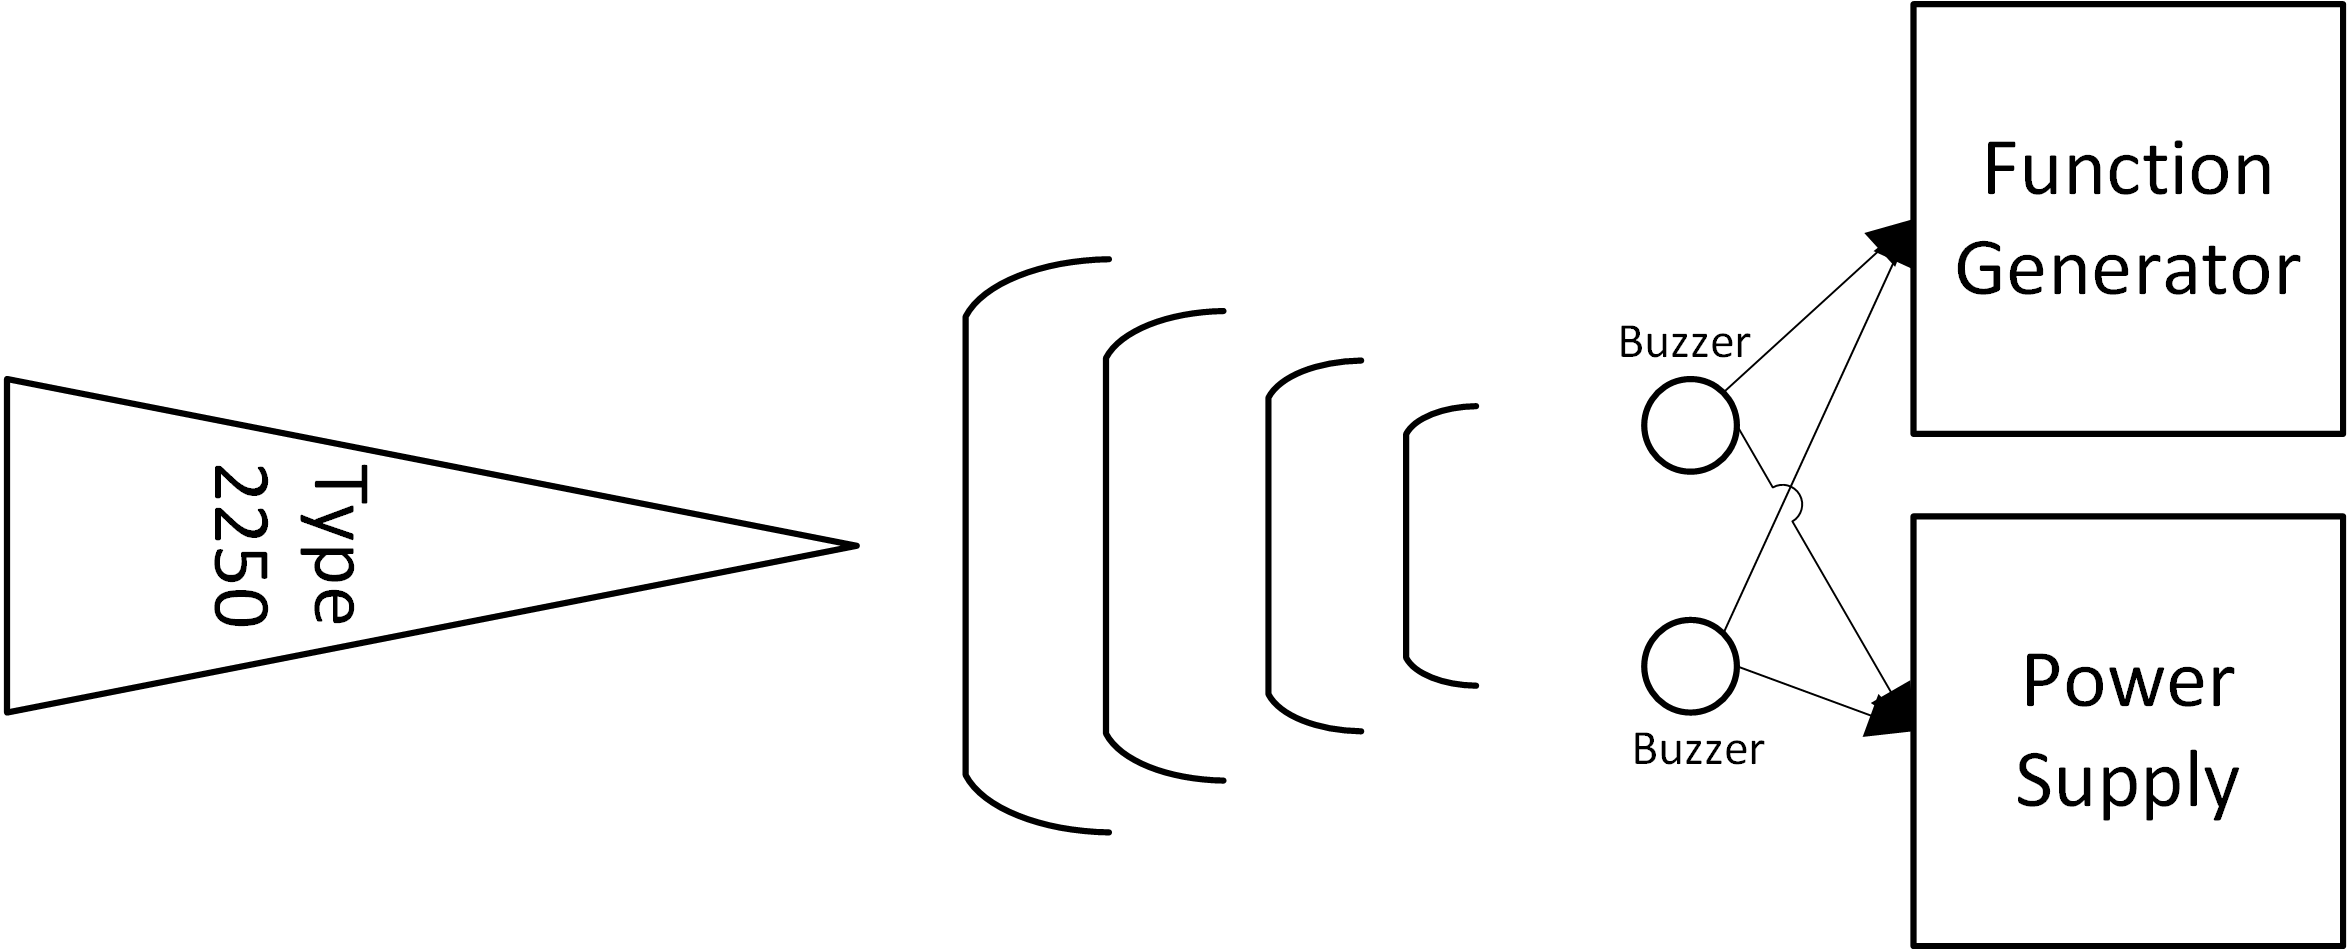
\includegraphics[width=0.7\linewidth]{Hardware/Pictures/Horn_test}
	\caption{Horn test setup}
	\label{fig:Horn_test}
\end{figure}

First tests were conducted on buzzer with product number KTG1205C\fxnote{husk ref} from manucfactor Kingstate. This were rated to provide a sound level of minimum 90dB (avg 94dB) at 10 cm. This specific model was chosen because of the small package size, their current consumption and relatively small weight weighing in at mere 2 gram per buzzer. This buzzers proved inadequate to provide the desired sound level required. It was tested to improve the sound level by parallel-coupling 2 buzzers, but the it was still not enough. Even with 2 sets of parallel-coupled buzzers, the sound level reached only 71 dB measured 4 meters away.

The next set of buzzers that were tested, was KPEG500\fxnote{husk ref} also from Kingstate. These buzzer were chosen from a sound level perspective and only that. This buzzer was much larger in size, current consumption was doubled and weighed roughly 15 times more at 27.8 gram. But they provided 104dB at 30cm at minimum, which was a much needed boost in deciBel. Testing with 2 of these buzzers resulted in a sound  level of 93 dB at 4 meters which is enough to fulfill the requirements. But as seen on the test setup it is not a 100\% accurate test and these measurements cannot be trusted completely but they show promise. \\
To perform a 100\% accurate test the speakers must be placed inside the vehicle and from there test if the sound level is adequate.

